\documentclass{beamer}

\mode<presentation>
{
  \usetheme{CambridgeUS}
  \setbeamercovered{transparent}
}

\usepackage{color}
\usepackage[ampersand]{easylist}
\usepackage[english]{babel}
\usepackage[latin1]{inputenc}
\usepackage{times}
\usepackage[T1]{fontenc} 
% Or whatever. Note that the encoding and the font should match. If T1
% does not look nice, try deleting the line with the fontenc.
\usepackage{amsmath}

\newcommand{\linespace}{\vskip 0.25cm}

\definecolor{MyForestGreen}{rgb}{0,0.7,0} 
\newcommand{\tableemph}[1]{{#1}}
\newcommand{\tablewin}[1]{\tableemph{#1}}
\newcommand{\tablemid}[1]{\tableemph{#1}}
\newcommand{\tablelose}[1]{\tableemph{#1}}

\definecolor{MyLightGray}{rgb}{0.6,0.6,0.6}
\newcommand{\tabletie}[1]{\color{MyLightGray} {#1}}

% The text in square brackets is the short version of your title and will be used in the
% header/footer depending on your theme.
\title[Applying EC to Robotics]{Applying Evolutionary Computation to Robotics}

% Sub-titles are optional - uncomment and edit the next line if you want one.
% \subtitle{Why does sub-tree crossover work?} 

% The text in square brackets is the short version of your name(s) and will be used in the
% header/footer depending on your theme.
\author[Schiller]{Adrian Thomas Schiller}

% The text in square brackets is the short version of your institution and will be used in the
% header/footer depending on your theme.
\institute[U of Minn, Morris]
{
  Division of Science and Mathematics \\
  University of Minnesota, Morris \\
  Morris, Minnesota, USA
}

% The text in square brackets is the short version of the date if you need that.
\date%[July '09, GECCO, Montr\'{e}al] % (optional)
{28 April 2014}

% Delete this, if you do not want the table of contents to pop up at
% the beginning of each subsection:
\AtBeginSection[]
{
  \begin{frame}<beamer>
    \frametitle{Outline}
    \tableofcontents[currentsection, hideothersubsections]
  \end{frame}
}

\begin{document}

\begin{frame}
  \titlepage
\end{frame}

\section{Overview}
\subsection*{The big picture}
\begin{frame}
  \frametitle{The big picture}

  \begin{columns}
  \begin{column}{0.6\textwidth}
  \begin{itemize}
    \item Robots are faced with difficult problems
        \item Evolutionary computation is a process which can can solve difficul
t problems in programming
        \item Since a robot interacts with the physical world, EC is slower by s
everal magnitudes
        \item It is possible to use EC to evolve robots
  \end{itemize}
  \end{column}
  \begin{column}{0.4\textwidth}
   \includegraphics[width=0.95\textwidth]{Illustrations/Empty_cocoon_crop_by_Bluedrakon_from_Flickr.jpg}
       \\
    \only{\tiny{Bluedrakon \\ \url{http://tr.im/pWUi} }}
  \end{column}
  \end{columns}
\end{frame}

%\subsection{Intro2}
%\begin{frame}
 % \frametitle{Introduce solving cases}
%\end{frame}

\section{Background}

\subsection{Evolutionary Computation}
\begin{frame}
  \frametitle{Evolutionary Computation}
 \begin{itemize}
  \item Evolutionary Computation (EC) is a problem solving technique which mimics natural selection
 
   \end{itemize}
\end{frame}
	
\begin{frame}
\frametitle{Evolutionary Computation: Requirements}
\begin{itemize}
  \item A population of candidates
  \item A fitness function
\end{itemize}
\end{frame}

\begin{frame}
\frametitle{Evolutionary Computation: Process}
 \begin{itemize}
  \item Candidates are evaluated
  \item The best performing candidates are selected
 \begin{itemize}
  \item Two candidates cross-over with one another
    \item Some candidates are subject to mutation
\end{itemize}
  \item This process repeats until the population is recreated
\end{itemize}
\end{frame}

\subsection{Genetic Algorithm}
\begin{frame}
  \frametitle{Genetic Algorithm}
\begin{itemize}
  \item Genetic Algorithms are a type of EC
  \item Candidates are represented as bit strings
\end{itemize}
\end{frame}

\begin{frame}

  \frametitle{Genetic Algorithm: Cross-over}
\begin{itemize}
  \item A Cross-over point is selected from two candidates. All bits are swapped beyond the point, creating two new candidates.
\end{itemize}
  \begin{columns}
  \begin{column}{0.5\textwidth}
\begin{itemize}
  \item Before:
\end{itemize}
\[
C_i=[ \textcolor{red}{1},  \textcolor{red}{0}, \textcolor{red}{1},  \textcolor{red}{0},|  \textcolor{red}{0},  \textcolor{red}{0}, \textcolor{red}{1}, \textcolor{red}{0}, \textcolor{red}{0}, \textcolor{red}{1} ]
\]
\[C_j=[  \textcolor{blue}{0}, \textcolor{blue}{0}, \textcolor{blue}{1}, \textcolor{blue}{1},| \textcolor{blue}{0}, \textcolor{blue}{1}, \textcolor{blue}{1}, \textcolor{blue}{0}, \textcolor{blue}{1}, \textcolor{blue}{0} ]
\]
\end{column}
 \begin{column}{0.5\textwidth}
\begin{itemize}
  \item After:
\end{itemize}
   \[
[ \textcolor{red}{1},  \textcolor{red}{0}, \textcolor{red}{1},  \textcolor{red}{0}, \textcolor{blue}{0}, \textcolor{blue}{1}, \textcolor{blue}{1}, \textcolor{blue}{0}, \textcolor{blue}{1}, \textcolor{blue}{0} ]
\]
\[ [  \textcolor{blue}{0}, \textcolor{blue}{0}, \textcolor{blue}{1}, \textcolor{blue}{1}, \textcolor{red}{0},  \textcolor{red}{0}, \textcolor{red}{1}, \textcolor{red}{0}, \textcolor{red}{0}, \textcolor{red}{1} ]
\]
  \end{column}
  \end{columns}
\end{frame}

\begin{frame}
  \frametitle{Genetic Algorithm: Candidate Manipulation}
\begin{itemize}
  \item Mutation:
\end{itemize}
\[
[ \textcolor{red}{1},  \textcolor{red}{0}, \textcolor{red}{1},  \textcolor{red}{0},  \textcolor{red}{0},  \textcolor{red}{0}, \textcolor{red}{1}, \textcolor{red}{0}, \textcolor{red}{1}, \textcolor{red}{1} ]
\]
\[[ \textcolor{red}{1},  \textcolor{red}{0}, \textcolor{red}{1},  \textcolor{red}{0},  \textcolor{red}{0},  \textcolor{red}{0}, \textcolor{red}{1}, \textcolor{red}{0}, \textcolor{blue}{0}, \textcolor{red}{1} ]
\]
\end{frame}

\subsection{``One Max'' Example}
\begin{frame}
  \frametitle{Example: ``One Max''}
\begin{itemize}
\item Goal: Evolve an array consisting of the most ones from 20 candidate arrays with 10 bits
\end{itemize}
\[
20 \left\{\begin{matrix}
[  1,~1,~1,~0,~ 0,~0,~1,~0,~0,~1] \\ %inkscape, omnigraphle, googledocs? (need pdf vector graphic)
[  0,~0,~1,~1,~ 0,~1,~1,~0,~1,~0] \\
\cdots\\
[  1 ,~0,~1,~0,~ 1,~1,~1,~0,~0,~0] 
\end{matrix}\right.
\]
\end{frame}

\begin{frame}
  \frametitle{Example: ``One Max''}
\begin{itemize}
\item The fitness function $F()$ is used to calculate the fitness of each candidate
\item In this case, the function counts the number of ones in the array
\end{itemize}

\[F([   \textcolor{red}{1},~\textcolor{red}{1},~ \textcolor{red}{1},~0,~ 0,~0,~\textcolor{red}{1},~ 0,~ 0,~ \textcolor{red}{1}]  ) = 6 \]%inkscape, omnigraphle, googledocs? (need pdf vector graphic)
\[F([  0 ,~0,~ \textcolor{red}{1},~ \textcolor{red}{1},~ 0,~ \textcolor{red}{1},~0,~0,~ \textcolor{red}{1},~0]) = 4\]
\[\cdots\]
\[F([   \textcolor{red}{1},~0,~ \textcolor{red}{1},~0,~  \textcolor{red}{1},~ \textcolor{red}{1},~ \textcolor{red}{1},~0,~0,~0]) = 5\]
\end{frame}

\begin{frame}
  \frametitle{Example: ``One Max''}
\begin{itemize}
\item The top 10 candidates are selected to create a new population
\item Top candidates are randomly selected to cross-over with one another
\end{itemize}

  \begin{columns}
  \begin{column}{0.5\textwidth}

\[
C_1=[ \textcolor{red}{1},  \textcolor{red}{1}, \textcolor{red}{1},  \textcolor{red}{0},|  \textcolor{red}{0},  \textcolor{red}{0}, \textcolor{red}{1}, \textcolor{red}{0}, \textcolor{red}{0}, \textcolor{red}{1} ]
\]
\[C_2=[  \textcolor{blue}{0}, \textcolor{blue}{0}, \textcolor{blue}{1}, \textcolor{blue}{1},| \textcolor{blue}{0}, \textcolor{blue}{1}, \textcolor{blue}{1}, \textcolor{blue}{0}, \textcolor{blue}{1}, \textcolor{blue}{0} ]
\]
\end{column}
 \begin{column}{0.5\textwidth}

   \[
C_x=[ \textcolor{red}{1},  \textcolor{red}{1}, \textcolor{red}{1},  \textcolor{red}{0}, \textcolor{blue}{0}, \textcolor{blue}{1}, \textcolor{blue}{1}, \textcolor{blue}{0}, \textcolor{blue}{1}, \textcolor{blue}{0} ]
\]
\[C_y = [  \textcolor{blue}{0}, \textcolor{blue}{0}, \textcolor{blue}{1}, \textcolor{blue}{1}, \textcolor{red}{0},  \textcolor{red}{0}, \textcolor{red}{1}, \textcolor{red}{0}, \textcolor{red}{0}, \textcolor{red}{1} ]
\]
  \end{column}
  \end{columns}
\end{frame}

\begin{frame}
  \frametitle{Example: ``One Max''}
\begin{itemize}
  \item Some created candidates may undergo mutation:
\end{itemize}
\[
C_x=[ \textcolor{red}{1},  \textcolor{red}{1}, \textcolor{red}{1},  \textcolor{red}{0}, \textcolor{red}{0}, \textcolor{red}{1}, \textcolor{red}{1}, \textcolor{red}{0}, \textcolor{red}{1}, \textcolor{red}{0} ]
\]
\[C_x'=[ \textcolor{red}{1},  \textcolor{red}{1}, \textcolor{red}{1},  \textcolor{red}{0}, \textcolor{blue}{1}, \textcolor{red}{1}, \textcolor{red}{1}, \textcolor{red}{0}, \textcolor{red}{1}, \textcolor{red}{0} ]
\]
\end{frame}

\begin{frame}
  \frametitle{Example: ``One Max''}
\begin{itemize}
  \item Once the population is recreated, the process repeats until eventually a limit is reached
  \item In this case, the limit would be time or finding an array of all 1's
\end{itemize}
\[
F([ \textcolor{red}{1},  \textcolor{red}{1}, \textcolor{red}{1}, 0, \textcolor{red}{1}, \textcolor{red}{1}, \textcolor{red}{1}, 0, \textcolor{red}{1}, 0 ]) = 7
\]
\[F([  0, 0, \textcolor{red}{1}, \textcolor{red}{1}, 0,  0, \textcolor{red}{1}, 0, 0, \textcolor{red}{1} ]) = 4
\]
\[\cdots\]
\[F([  \textcolor{red}{1}, 0, \textcolor{red}{1}, \textcolor{red}{1}, 0,  \textcolor{red}{1}, 0, 0, \textcolor{red}{1}, \textcolor{red}{1} ]) = 6
\]
\end{frame}

\subsection{Artificial Neural Networks}
\begin{frame}
  \frametitle{Artificial Neural Networks (ANN)}
\begin{columns}
  \begin{column}{0.5\textwidth}
\begin{itemize}
\item  ANNs are a collection of nodes with weighted vertices.
\item 
\end{itemize}
\end{column}
\begin{column}{0.5\textwidth}
 \includegraphics[width=0.95\textwidth]{Illustrations/cr2.pdf}
       \\
    \only{\tiny{Bluedrakon \\ \url{http://tr.im/pWUi} }}
\end{column}
\end{columns}
\end{frame}

\section{Research Cases}

\subsection{Station Keeping Robot}
\begin{frame}
  \frametitle{Station Keeping Robot}
\begin{center}
 \includegraphics[width=0.95\textwidth]{Illustrations/sr2.pdf}
       \\
    \only{\tiny{Bluedrakon \\ \url{http://tr.im/pWUi} }}
\end{center}
\begin{itemize}
\item \large The station keeping robot was developed by Moore $et~al.$ 
\item \large Goal: to maintain position in a body of water
\end{itemize}
\end{frame}

\begin{frame}
  \frametitle{Station Keeping Robot}
\begin{center}
 \includegraphics[width=0.57\textwidth]{Illustrations/sr4.pdf}
       \\
    \only{\tiny{Bluedrakon \\ \url{http://tr.im/pWUi} }}
\end{center}

\end{frame}

\subsection{WalkingRobot}
\begin{frame}
  \frametitle{Walking Robot}

\begin{columns}
  \begin{column}{0.5\textwidth}
\begin{itemize}
\item  Farchy $et~al.$ modified the code of the Aldebaran Nao robot
\item Goal: to increase walking speed
\end{itemize}
\end{column}
\begin{column}{0.5\textwidth}
 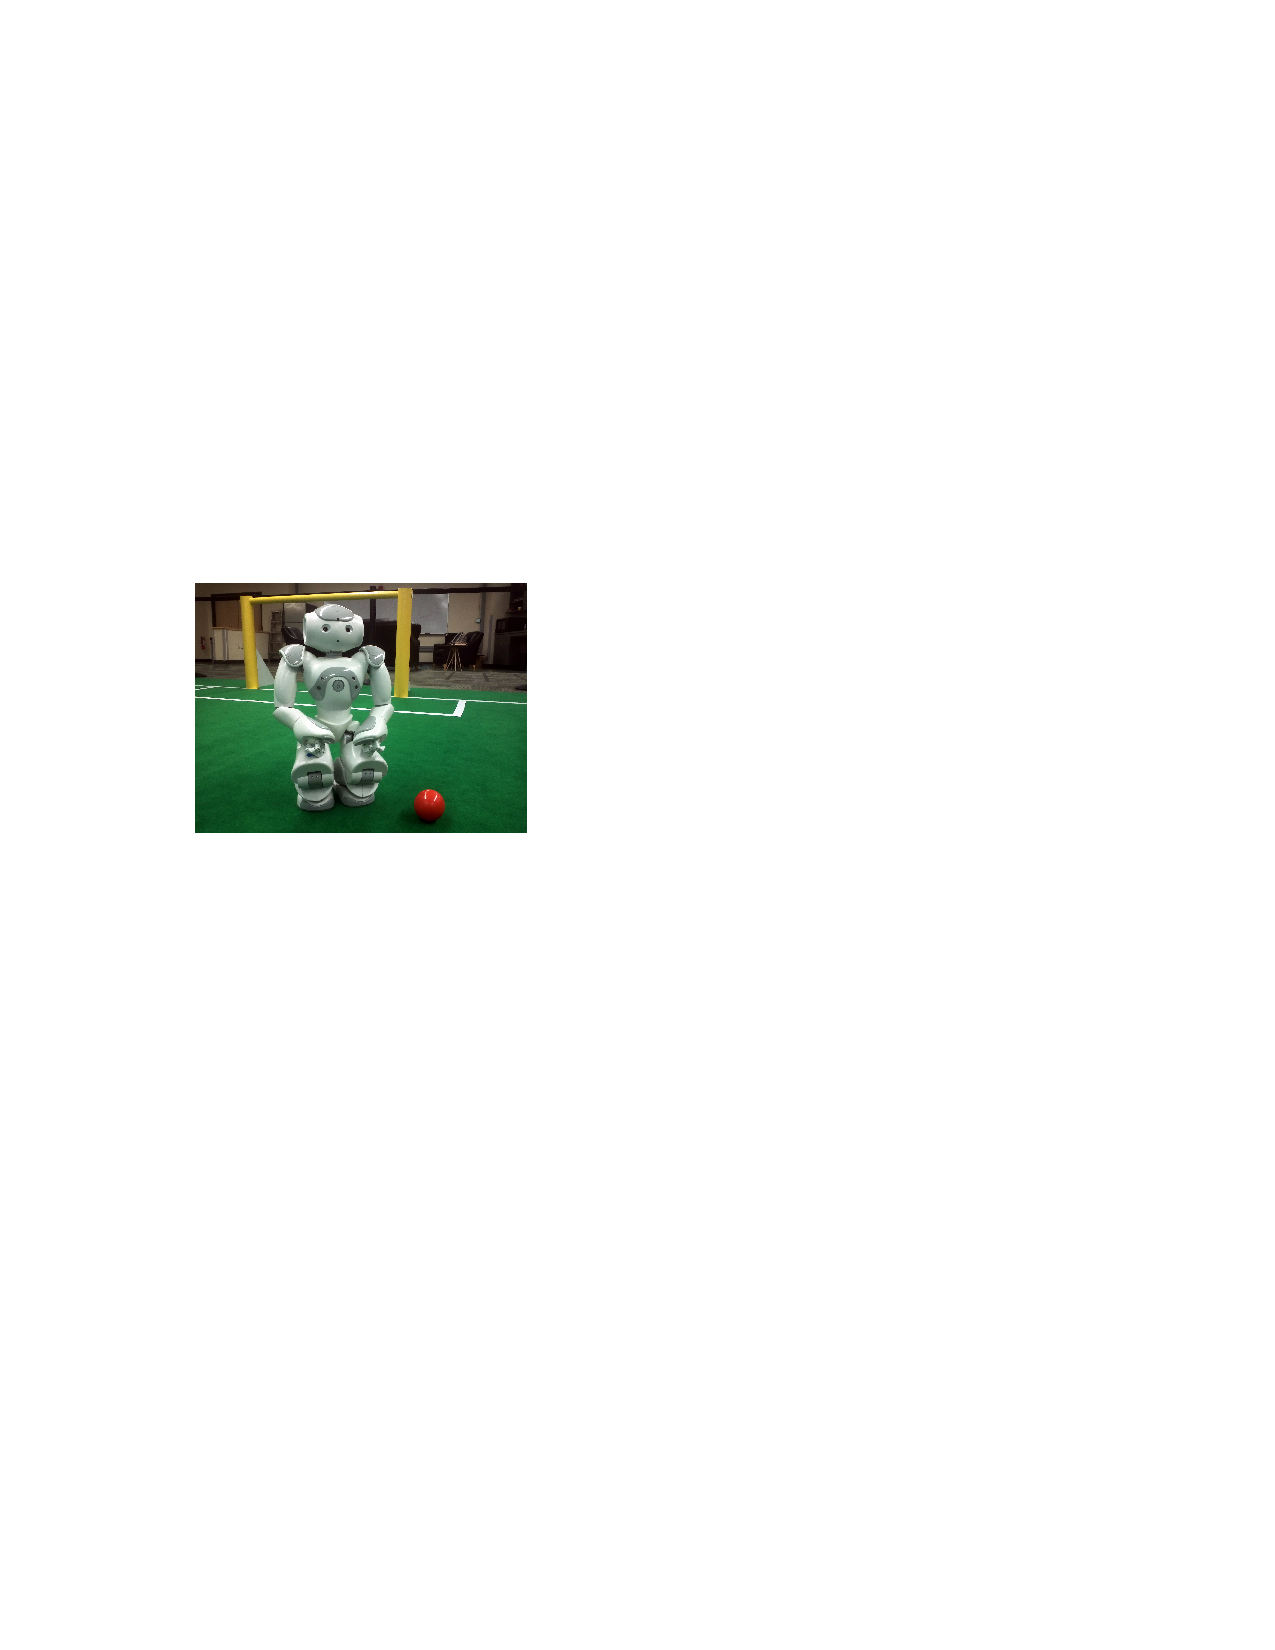
\includegraphics[width=0.95\textwidth]{Illustrations/wr1.pdf}
       \\
    \only{\tiny{Bluedrakon \\ \url{http://tr.im/pWUi} }}
\end{column}
\end{columns}
\end{frame}

\subsection{CoordRobot}
\begin{frame}
  \frametitle{Coordinate Tracking Robot}
\begin{columns}
  \begin{column}{0.5\textwidth}
\begin{itemize}
\item  Pretorius $et~al.$ created a Lego Mindstorms robot
\item Goal: to evolve an internal navigation controller
\end{itemize}
\end{column}
\begin{column}{0.5\textwidth}
 \includegraphics[width=0.95\textwidth]{Illustrations/cr1.pdf}
       \\
    \only{\tiny{Bluedrakon \\ \url{http://tr.im/pWUi} }}
\end{column}
\end{columns}
\end{frame}

\section{Simulation}

\subsection{Station Keeping Robot: Simulation}
\begin{frame}
  \frametitle{Station Keeping Robot: Simulation}
\begin{center}
 \includegraphics[width=0.7\textwidth]{Illustrations/sr6.pdf}
       \\
    \only{\tiny{Bluedrakon \\ \url{http://tr.im/pWUi} }}
\end{center}
\end{frame}

\subsection{SimWalkingRobot}
\begin{frame}
  \frametitle{Walking Robot: Simulation}
\begin{center}
 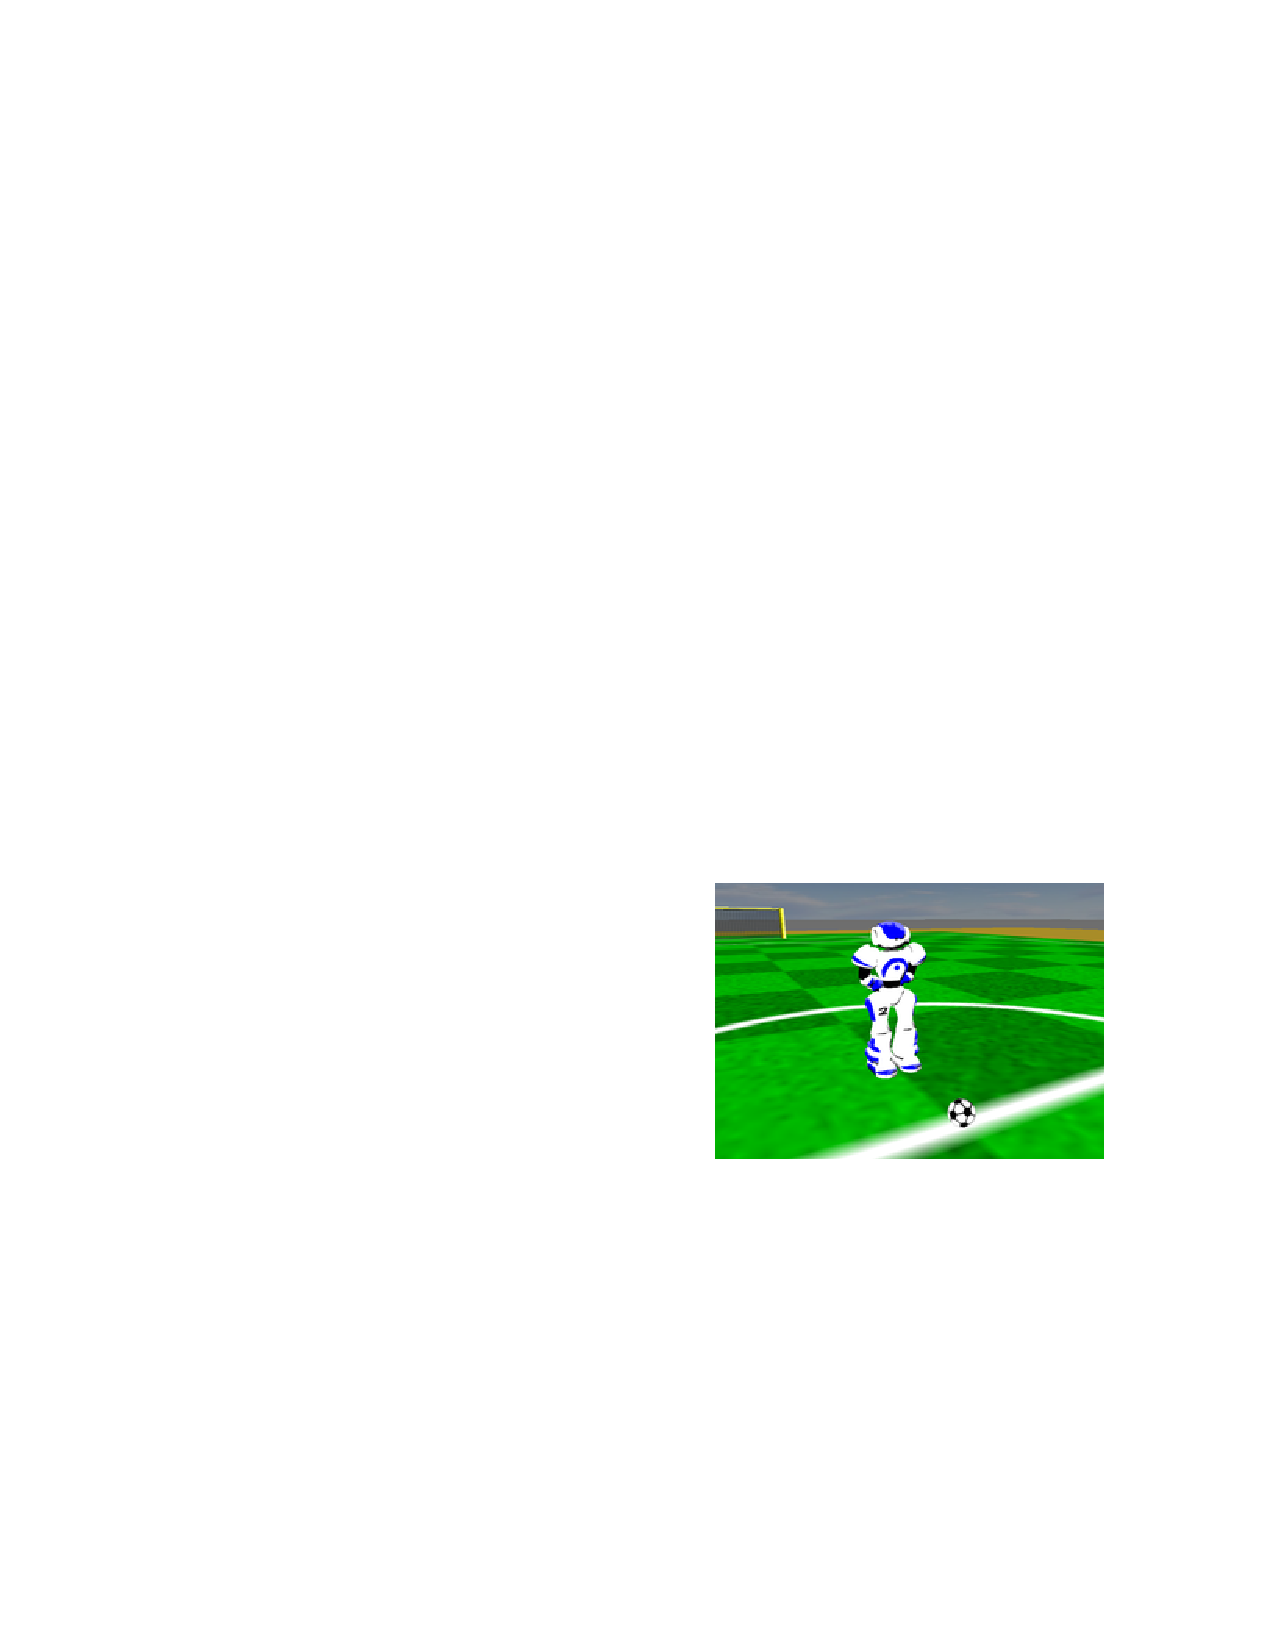
\includegraphics[width=0.7\textwidth]{Illustrations/wr2.pdf}
       \\
    \only{\tiny{Bluedrakon \\ \url{http://tr.im/pWUi} }}
\end{center}
\end{frame}

\subsection{SimCoordRobot}
\begin{frame}
  \frametitle{Coordinate Tracking Robot: Simulation}

\end{frame}

\subsection{SimCoordRobot}
\begin{frame}
  \frametitle{Coordinate Tracking Robot}
\end{frame}

\section{EvolutionaryProcess}

\subsection{Station Keeping Robot: Evolutionary Process}
\begin{frame}
  \frametitle{Swimming Robot: Evolutionary Process}
%Trials (45 sec)
%Neural Network (45 sec)
%Fitness function (45 sec)
%Tweaks to fitness function (1 min)
\end{frame}

\subsection{EPWalkingRobot: Evolutionary Process}
\begin{frame}
  \frametitle{Walking Robot: Simulation}
%Fitness function (1 min)
%GSL (2 min)
\end{frame}

\subsection{EPCoordRobot: Evolutionary Process}
\begin{frame}
  \frametitle{Coordinate Tracking Robot: Simulation}
%Explain commands (45 sec)
%Neural Network (45 sec)
%Fitness function (1 min)
%Explain nav controller (1:30 min)
\end{frame}

\section{Results}
\subsection{Station Keeping Robot: Results} %http://y2u.be/UufbnEGFwV4
\begin{frame}
  \frametitle{Station Keeping Robot: Results}
  \begin{center}
  \includegraphics[width=0.75\textwidth]{Illustrations/sr1.pdf}
       \\
    \only{\tiny{Moore et al. }}
    \end{center}
  \begin{itemize}
    \item Each trial had a candidate which successfully maintained the position
        \item When the flow was coming from behind, the evolved candidate would flip end-over-head to orient itself (http://y2u.be/UufbnEGFwV4)
  \end{itemize}
\end{frame}

\subsection{Walking Robot: Results}
\begin{frame}
  \frametitle{Walking Robot: Results}
\end{frame}

\begin{frame}
  \frametitle{Walking Robot: Results}

\begin{center}
 \includegraphics[width=0.7\textwidth]{Illustrations/wr4.pdf}
       \\
    \only{\tiny{Bluedrakon \\ \url{http://tr.im/pWUi} }}
\end{center}
\end{frame}

\subsection{ResultsCoordRobot}
\begin{frame}
  \frametitle{Coordinate Tracking Robot: Results}
\end{frame}

\begin{frame}
  \frametitle{Coordinate Tracking Robot: Results}
\begin{center}
 \includegraphics[width=0.7\textwidth]{Illustrations/cr3.pdf}
       \\
    \only{\tiny{Bluedrakon \\ \url{http://tr.im/pWUi} }}
\end{center}
\end{frame}

\section{Conclusion}
\subsection{}
\begin{frame}
  \frametitle{Conclusion}
  \begin{itemize}
\item By using a simulation, the evolutionary process can occur at a significantly faster rate
\item Evolutionary robotics could be applied if:
 \begin{itemize}
\item the robotics problem is well defined, %solution is not apparent?
\item the robot and environment can be simulated,
\item and the simulated robot's success can be quantified
\end{itemize}
\end{itemize}
\end{frame}

\section{Questions and Acknowledgments}
\subsection{}
\begin{frame}
  \frametitle{}
  Any Questions?

Thank you to Nic McPhee, Elena Machkasova, and Alex Jarvis for invaluable feedback
\end{frame}

\end{document}
